\documentclass{beamer}
\usepackage[latin1]{inputenc}
\usepackage{amssymb}
\usepackage{subfigure}
\usetheme{Warsaw}
\title[The Dependence of Planning Horizon on Model Accuracy]{The Dependence of Effective Planning Horizon on Model Accuracy}
\author[]{David Abel  \and Enrique Areyan \\ Kavosh Asadi  \and David Hershkowitz}
\date{December 15, 2015}
\begin{document}

% Title Slide
\begin{frame}
\titlepage
\end{frame}

% Dave/Ellis vote we don't include an outline since it's only 5 minutes.
%% Slide: What is the point?
\begin{frame}{Outline}
\begin{enumerate}
	\item What is the point?
	\item Value Iteration Story
	\item Value Iteration Results
	\item UCT Story
	\item UCT Results
\end{enumerate}
\end{frame}

% Slide: What is the point?
\begin{frame}{What is the Point?}
\centering
Planning depth should be determined proportionally to model accuracy
\begin{figure}
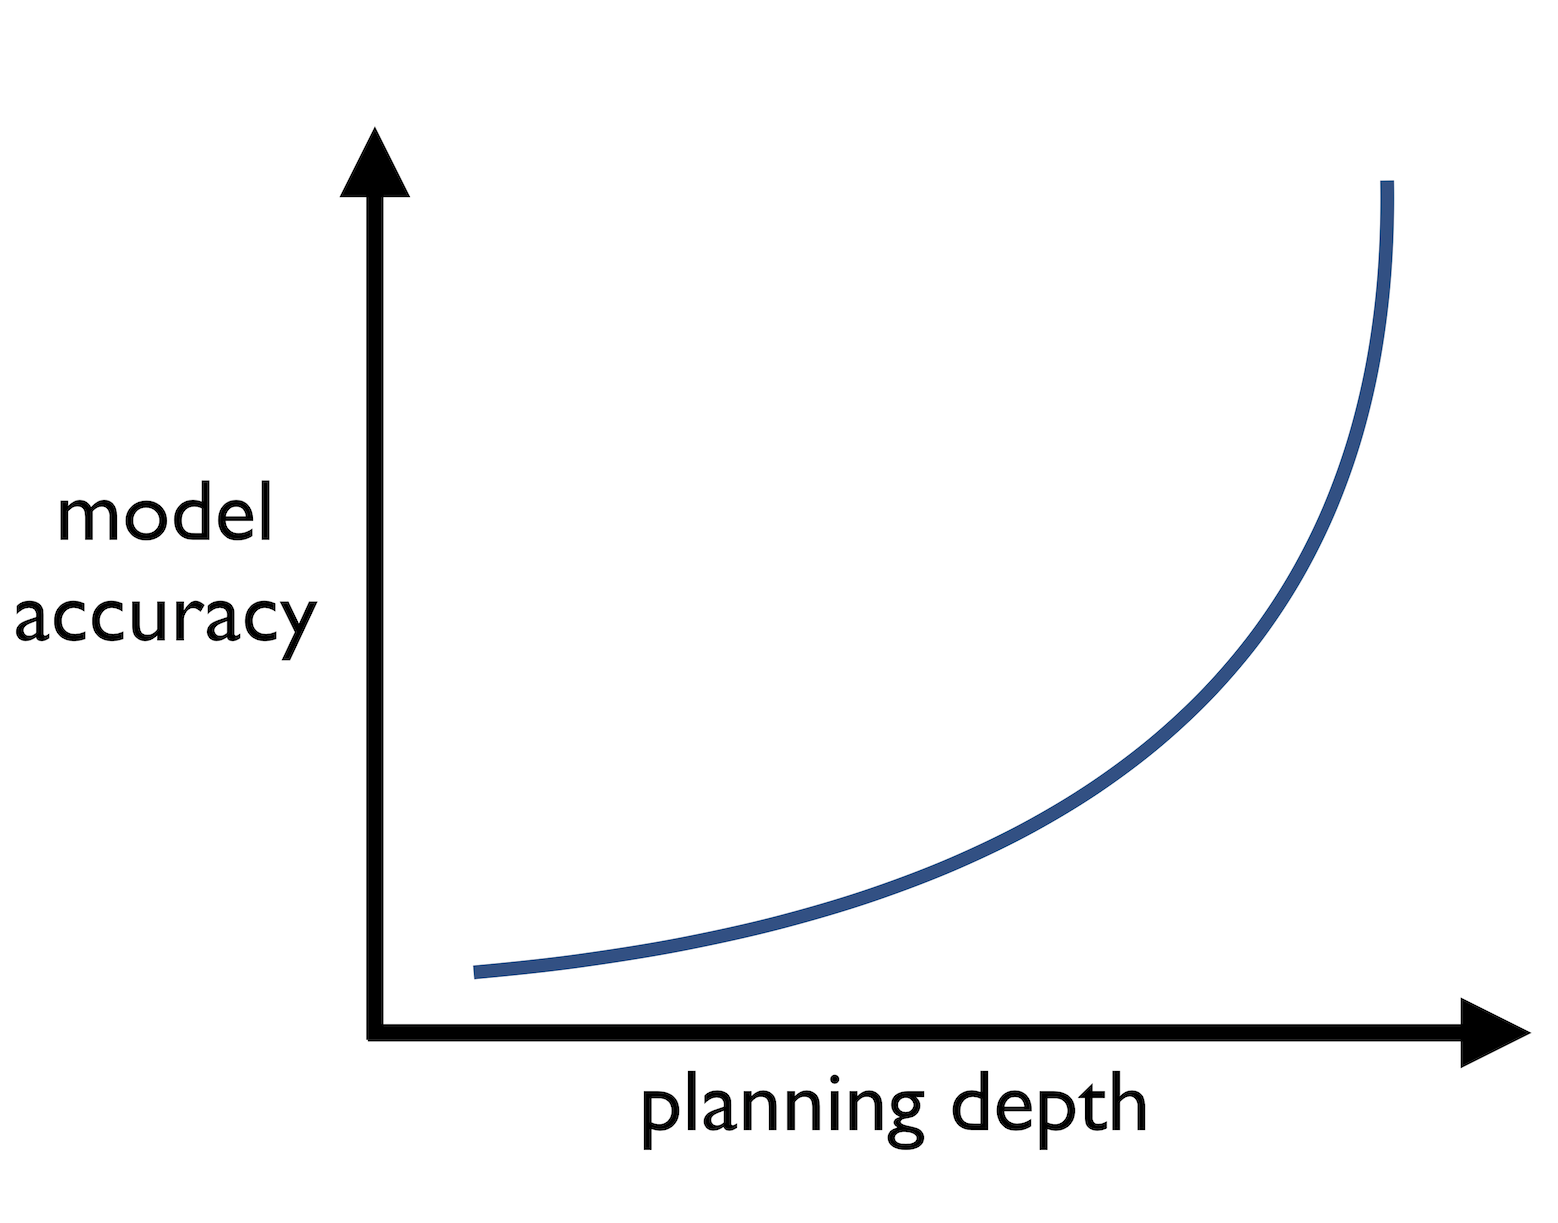
\includegraphics[page=1,width=.5\textwidth]{WhatIsThePoint.png}
\end{figure}
%An Innacurate
%With limited data 
%With an inaccurate model use a low planning Depth
\end{frame}


% Slide: RandomMDP Story
\begin{frame}{Value Iteration Story}
The evaluation is performed on a MDP designed by the authors, called RandomMDP, specified as:\vspace{8mm}
\begin{enumerate}
\setlength\itemsep{1em}
\item 10 states, 2 actions 
\item For each state-action pair, the agent can transition to 5 possible next states chosen uniformly.
The transition probability assigned to each next state  $\sim$ uniform$(0,1)$. 
\item Rewards \mbox{$\sim$ uniform$(0,1)$}, sample rewards have additive Gaussian noise
\item $\gamma_{eval} = 0.99$ and $\gamma_{plan} = 0.3,0.66, \text{and } 0.99$
\end{enumerate}

\end{frame}

\begin{frame}{Value Iteration Evaluation approach}
\begin{figure}
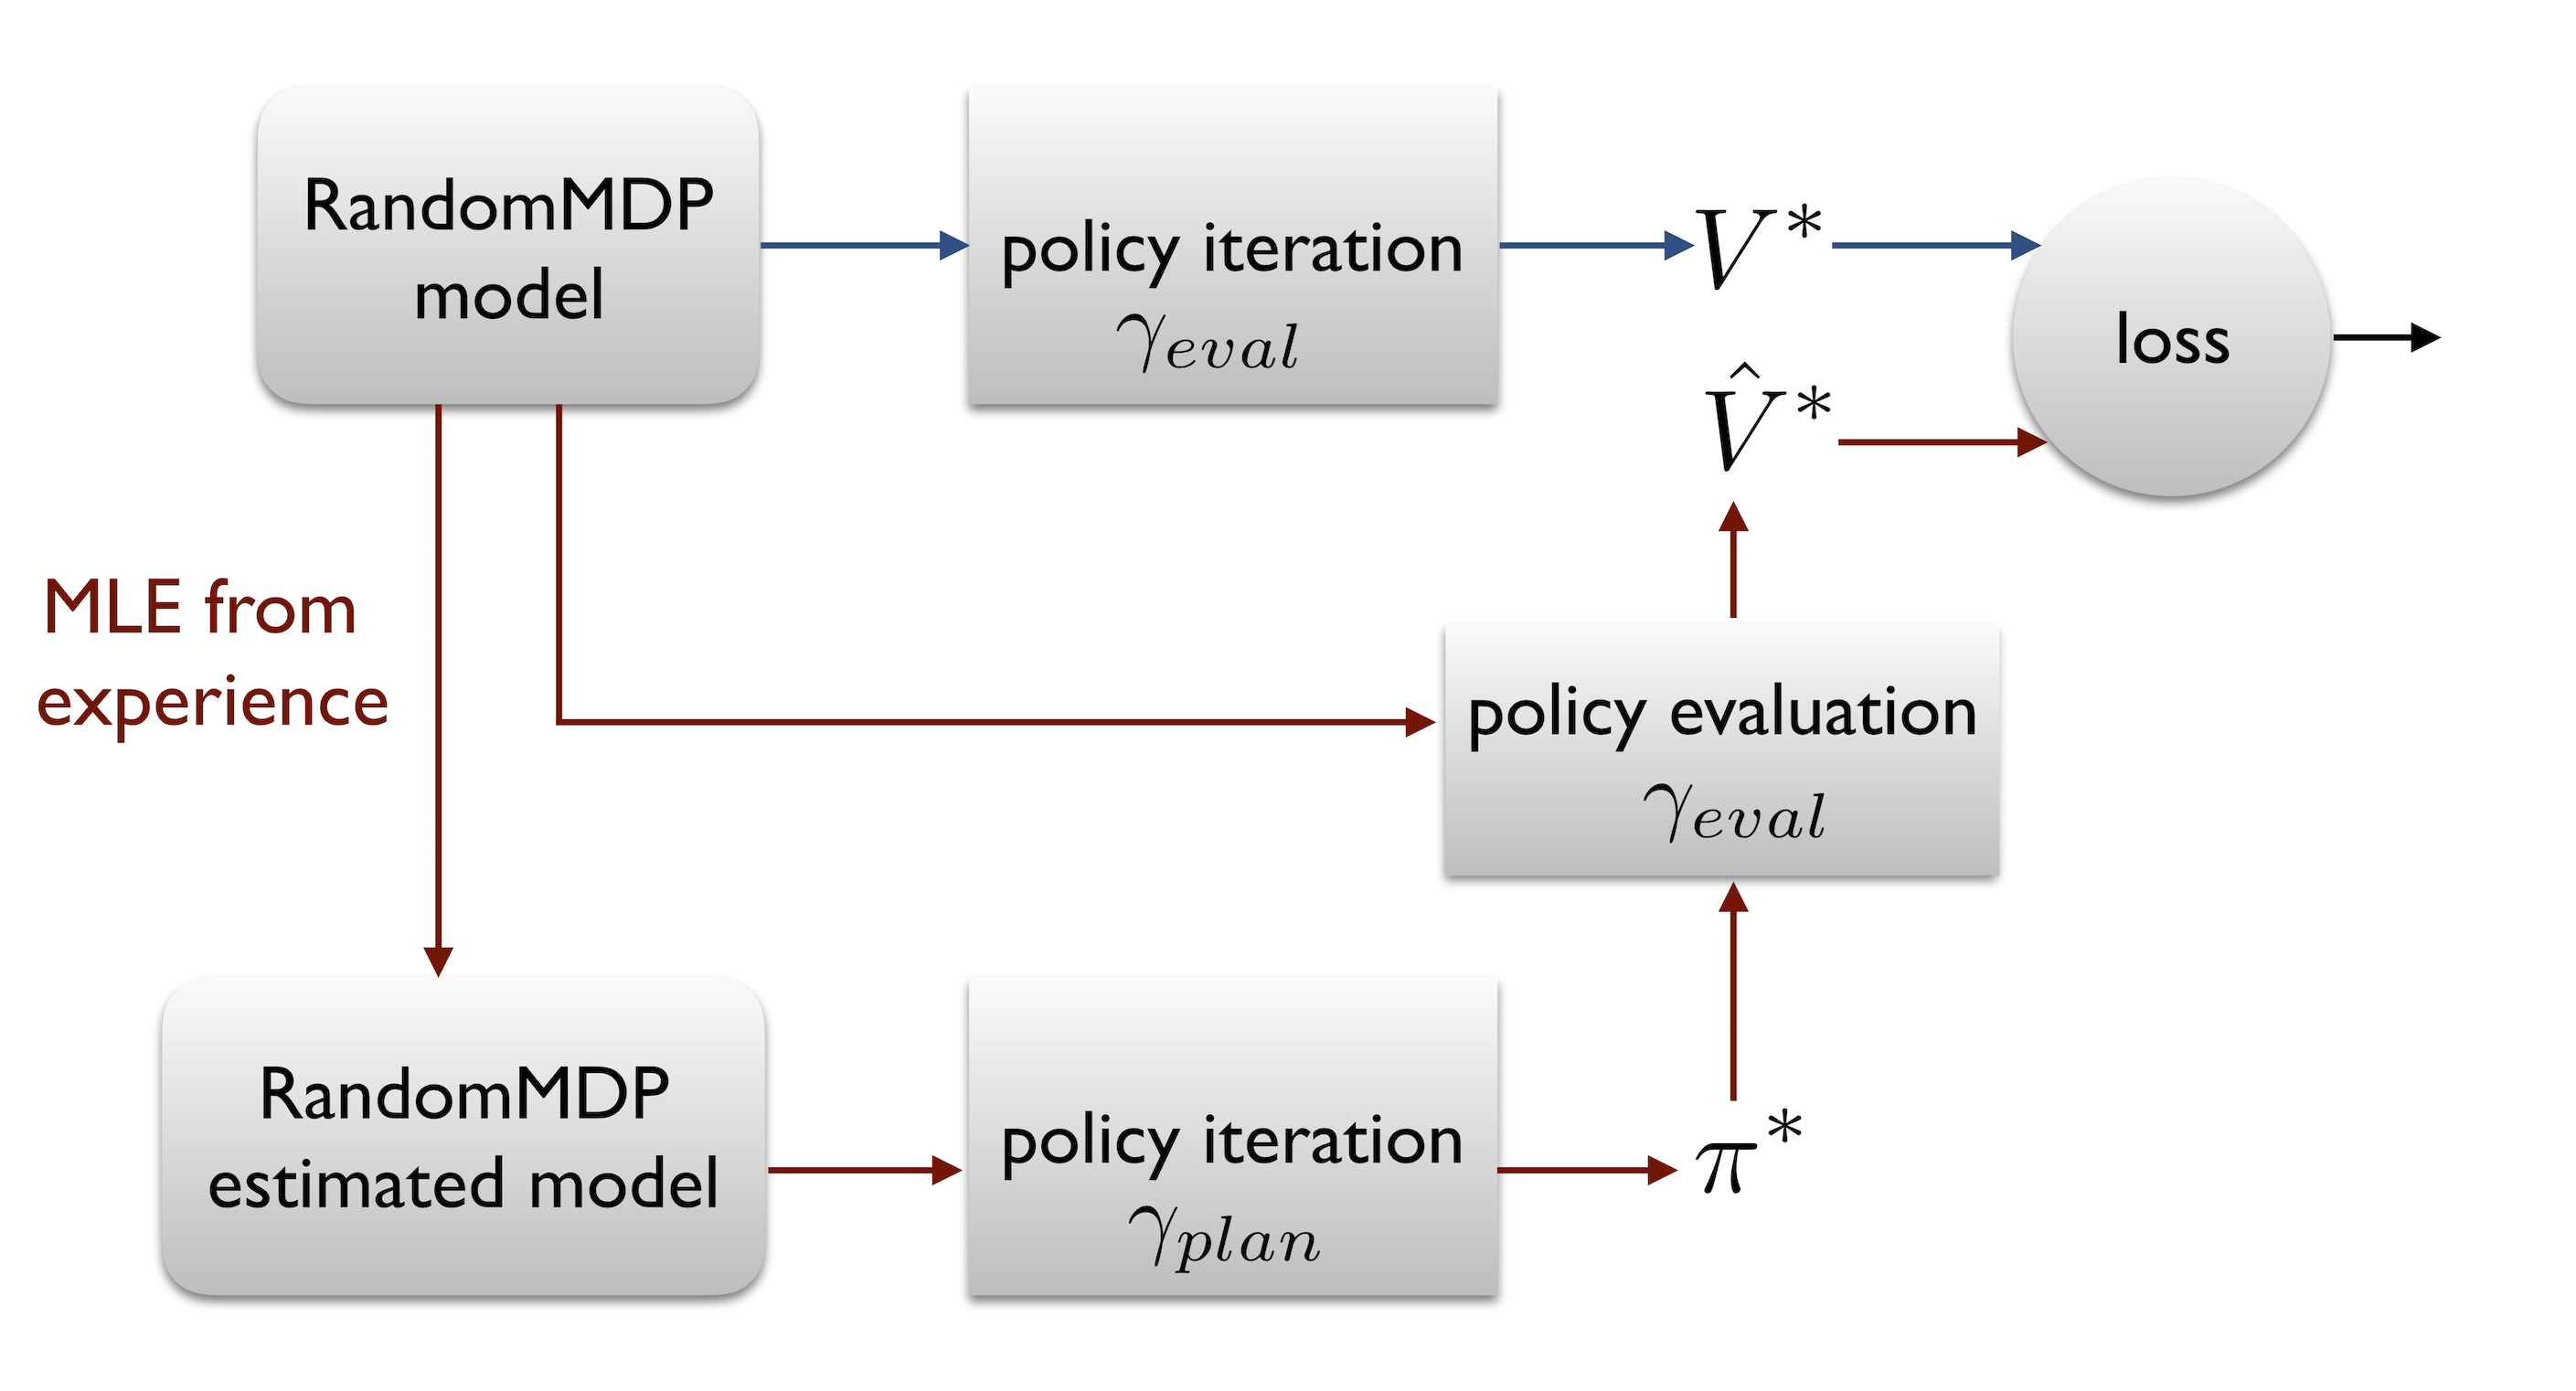
\includegraphics[page=1,width=1\textwidth]{RandomMDPEvaluation.png}
\end{figure}


\end{frame}

% Slide: RandomMDP Results
\begin{frame}{Value Iteration Results}
\begin{tabular}{cc}
our results & their results \\
	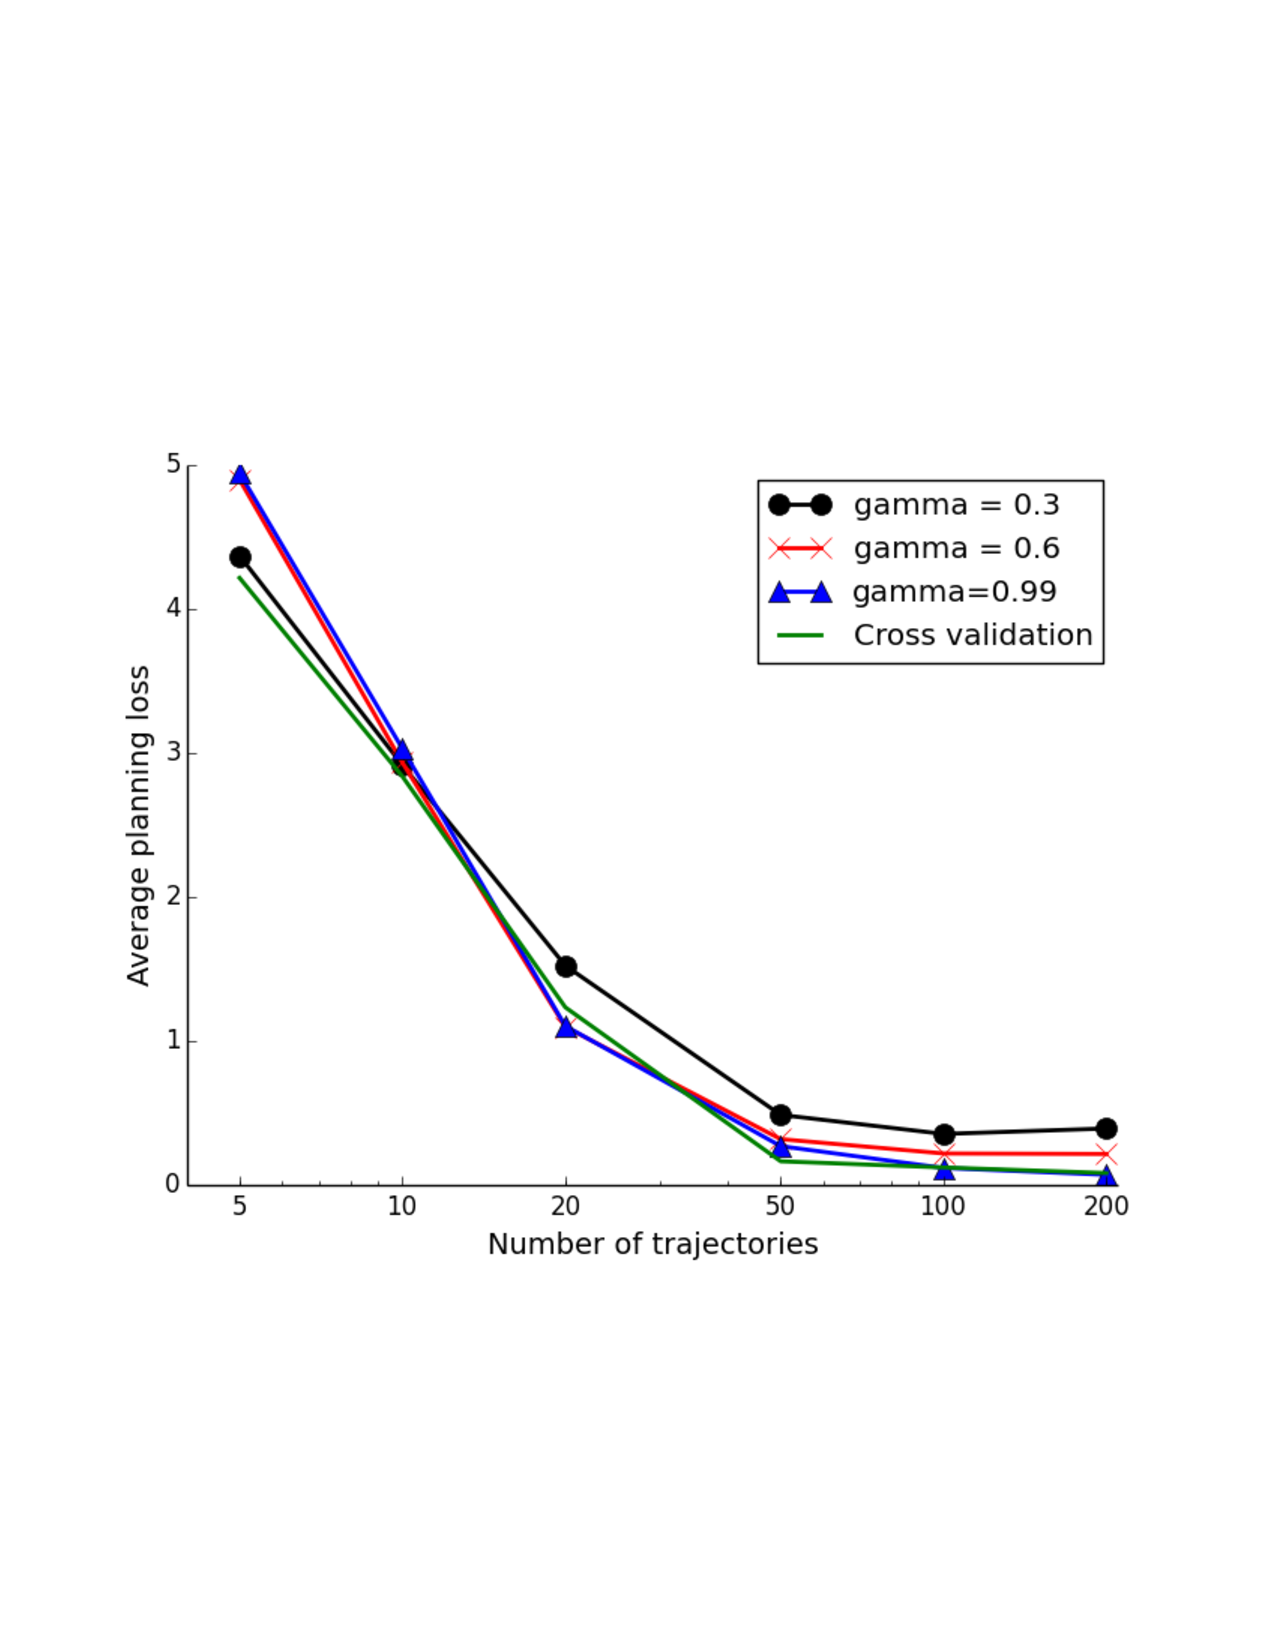
\includegraphics[page=1,height=.55\textheight,width=.5\textwidth]{../results/figure_2.pdf} &
	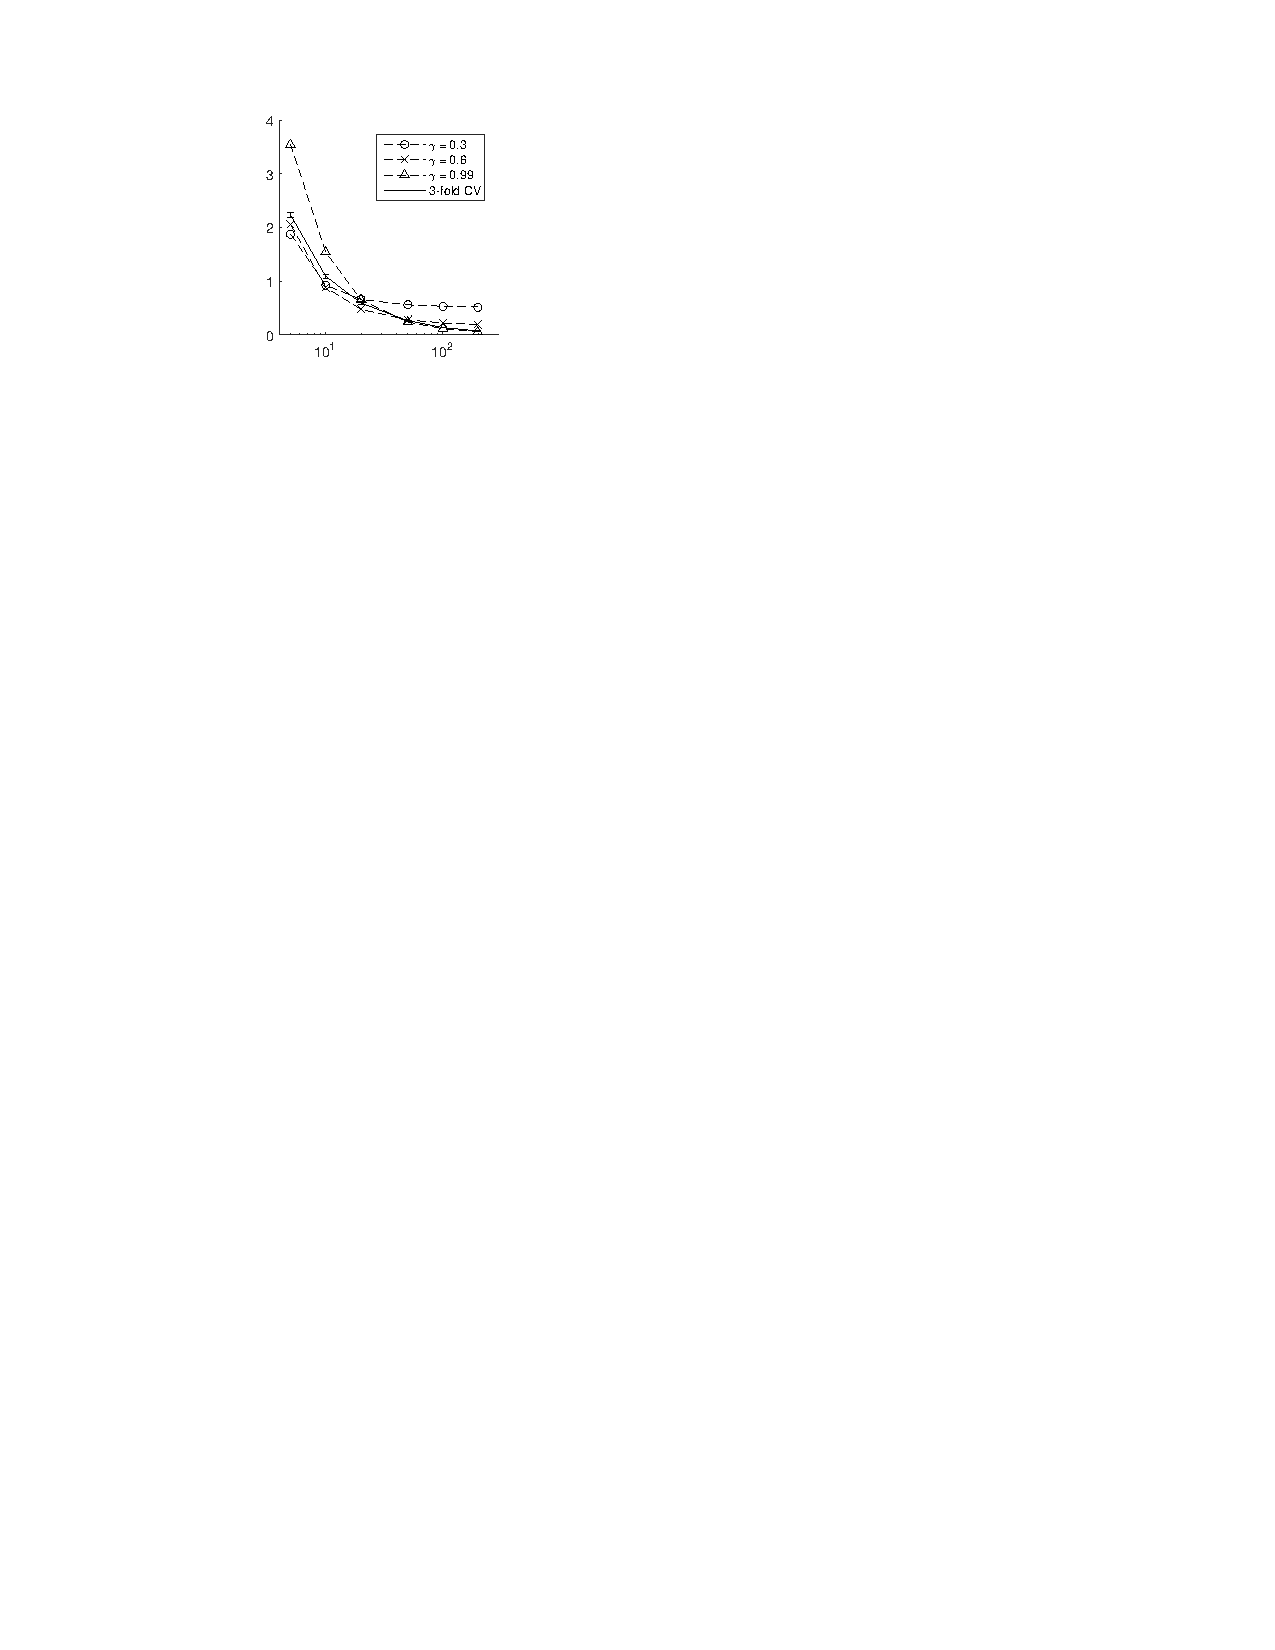
\includegraphics[page=1,width=.41\textwidth]{../results/originalCV.pdf}
\end{tabular}
\end{frame}

\begin{frame}{Value Iteration Reproducibility Discussion}
\begin{itemize}\setlength\itemsep{1em}
\item Definition of RandomMDP
\item Loss function 
\item Plot readability 
\end{itemize}
\end{frame}


% Slide: UCT Story
\begin{frame}{UCT Story}
UCT: 
\begin{itemize}
\item UCB
\item Monte Carlo Planning
% \item Planning Depth and $\gamma$
\end{itemize}

Experiments:
\begin{itemize}
\item Rock Sample Domain
\item Comparing UCT performance with different planning depths.
\end{itemize}
\end{frame}

% Slide: UCT Story
\begin{frame}{Rock Sample Domain}

\begin{figure}
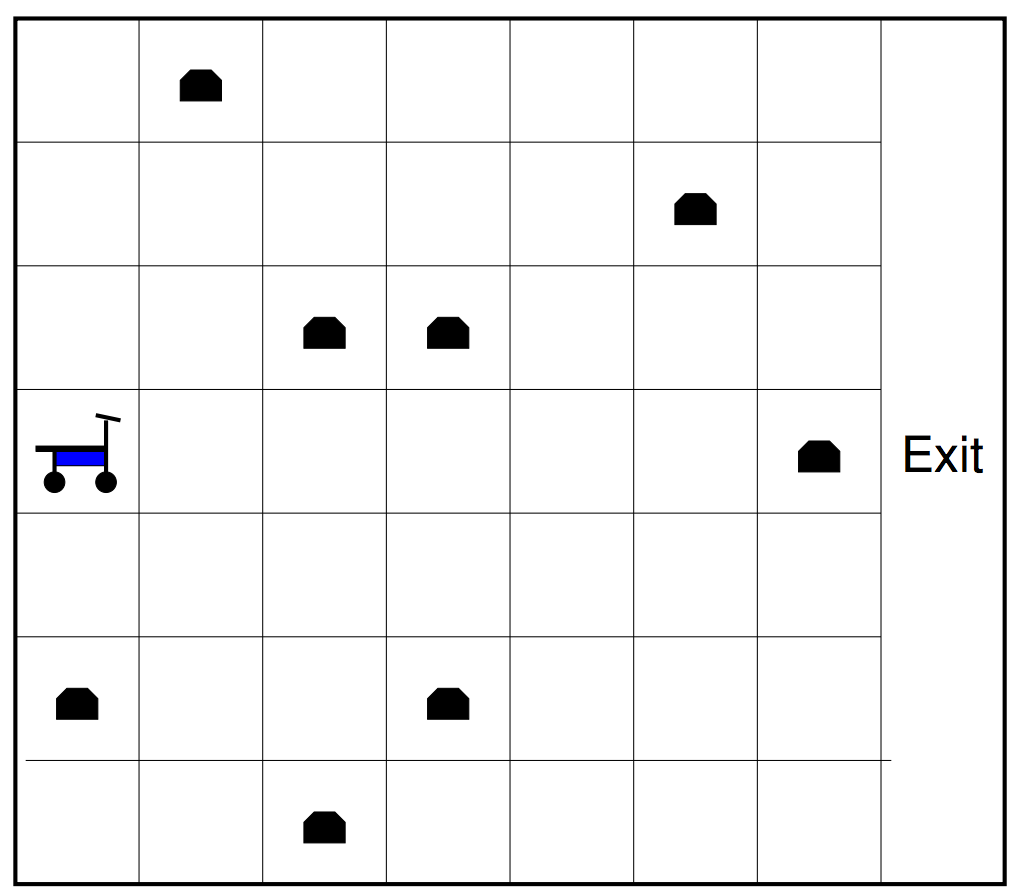
\includegraphics[page=1,height=.55\textheight,width=.5\textwidth]{rock_sample_domain.png}
\end{figure}


\end{frame}

% UCT Results
\begin{frame}{UCT Results}
\begin{figure}[h]
\centering
\subfigure[Our results]{
\label{fig: UCTOurResults}
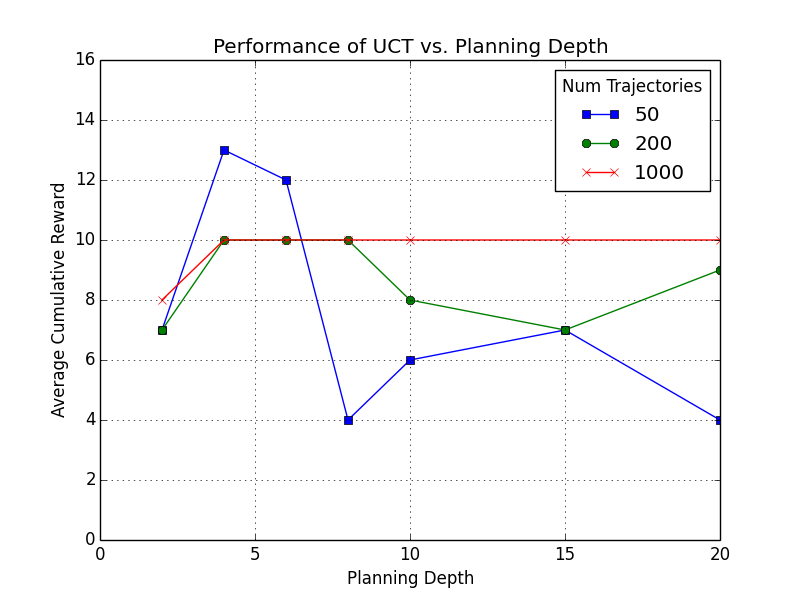
\includegraphics[page=1,width=.48\textwidth]{../results/rock_sample_results.png}}
\hspace{1mm}
\subfigure[Their results]{
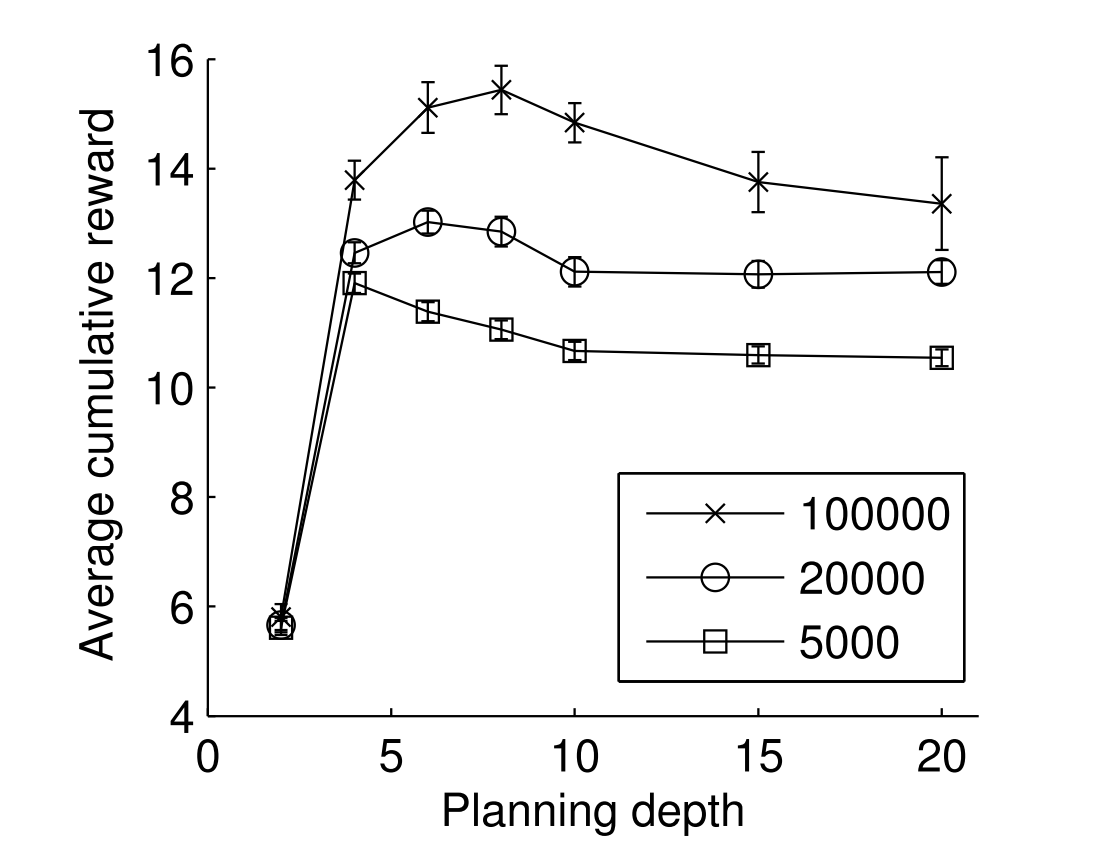
\includegraphics[page=1,width=.46\textwidth]{../results/figure_6.png}}
\end{figure}
\end{frame}

% Slide: Reproducbility Discussion
\begin{frame}{UCT Reproducibility Discussion}
\begin{itemize}\setlength\itemsep{1em}
\item Ambiguities of UCT
\item Ambiguities of Rock Sample
\item Computational Limitations
\end{itemize}
\end{frame}












\end{document}
